\begin{tikzpicture}

	\onslide<1->{ \node[] (input_taj) 
		{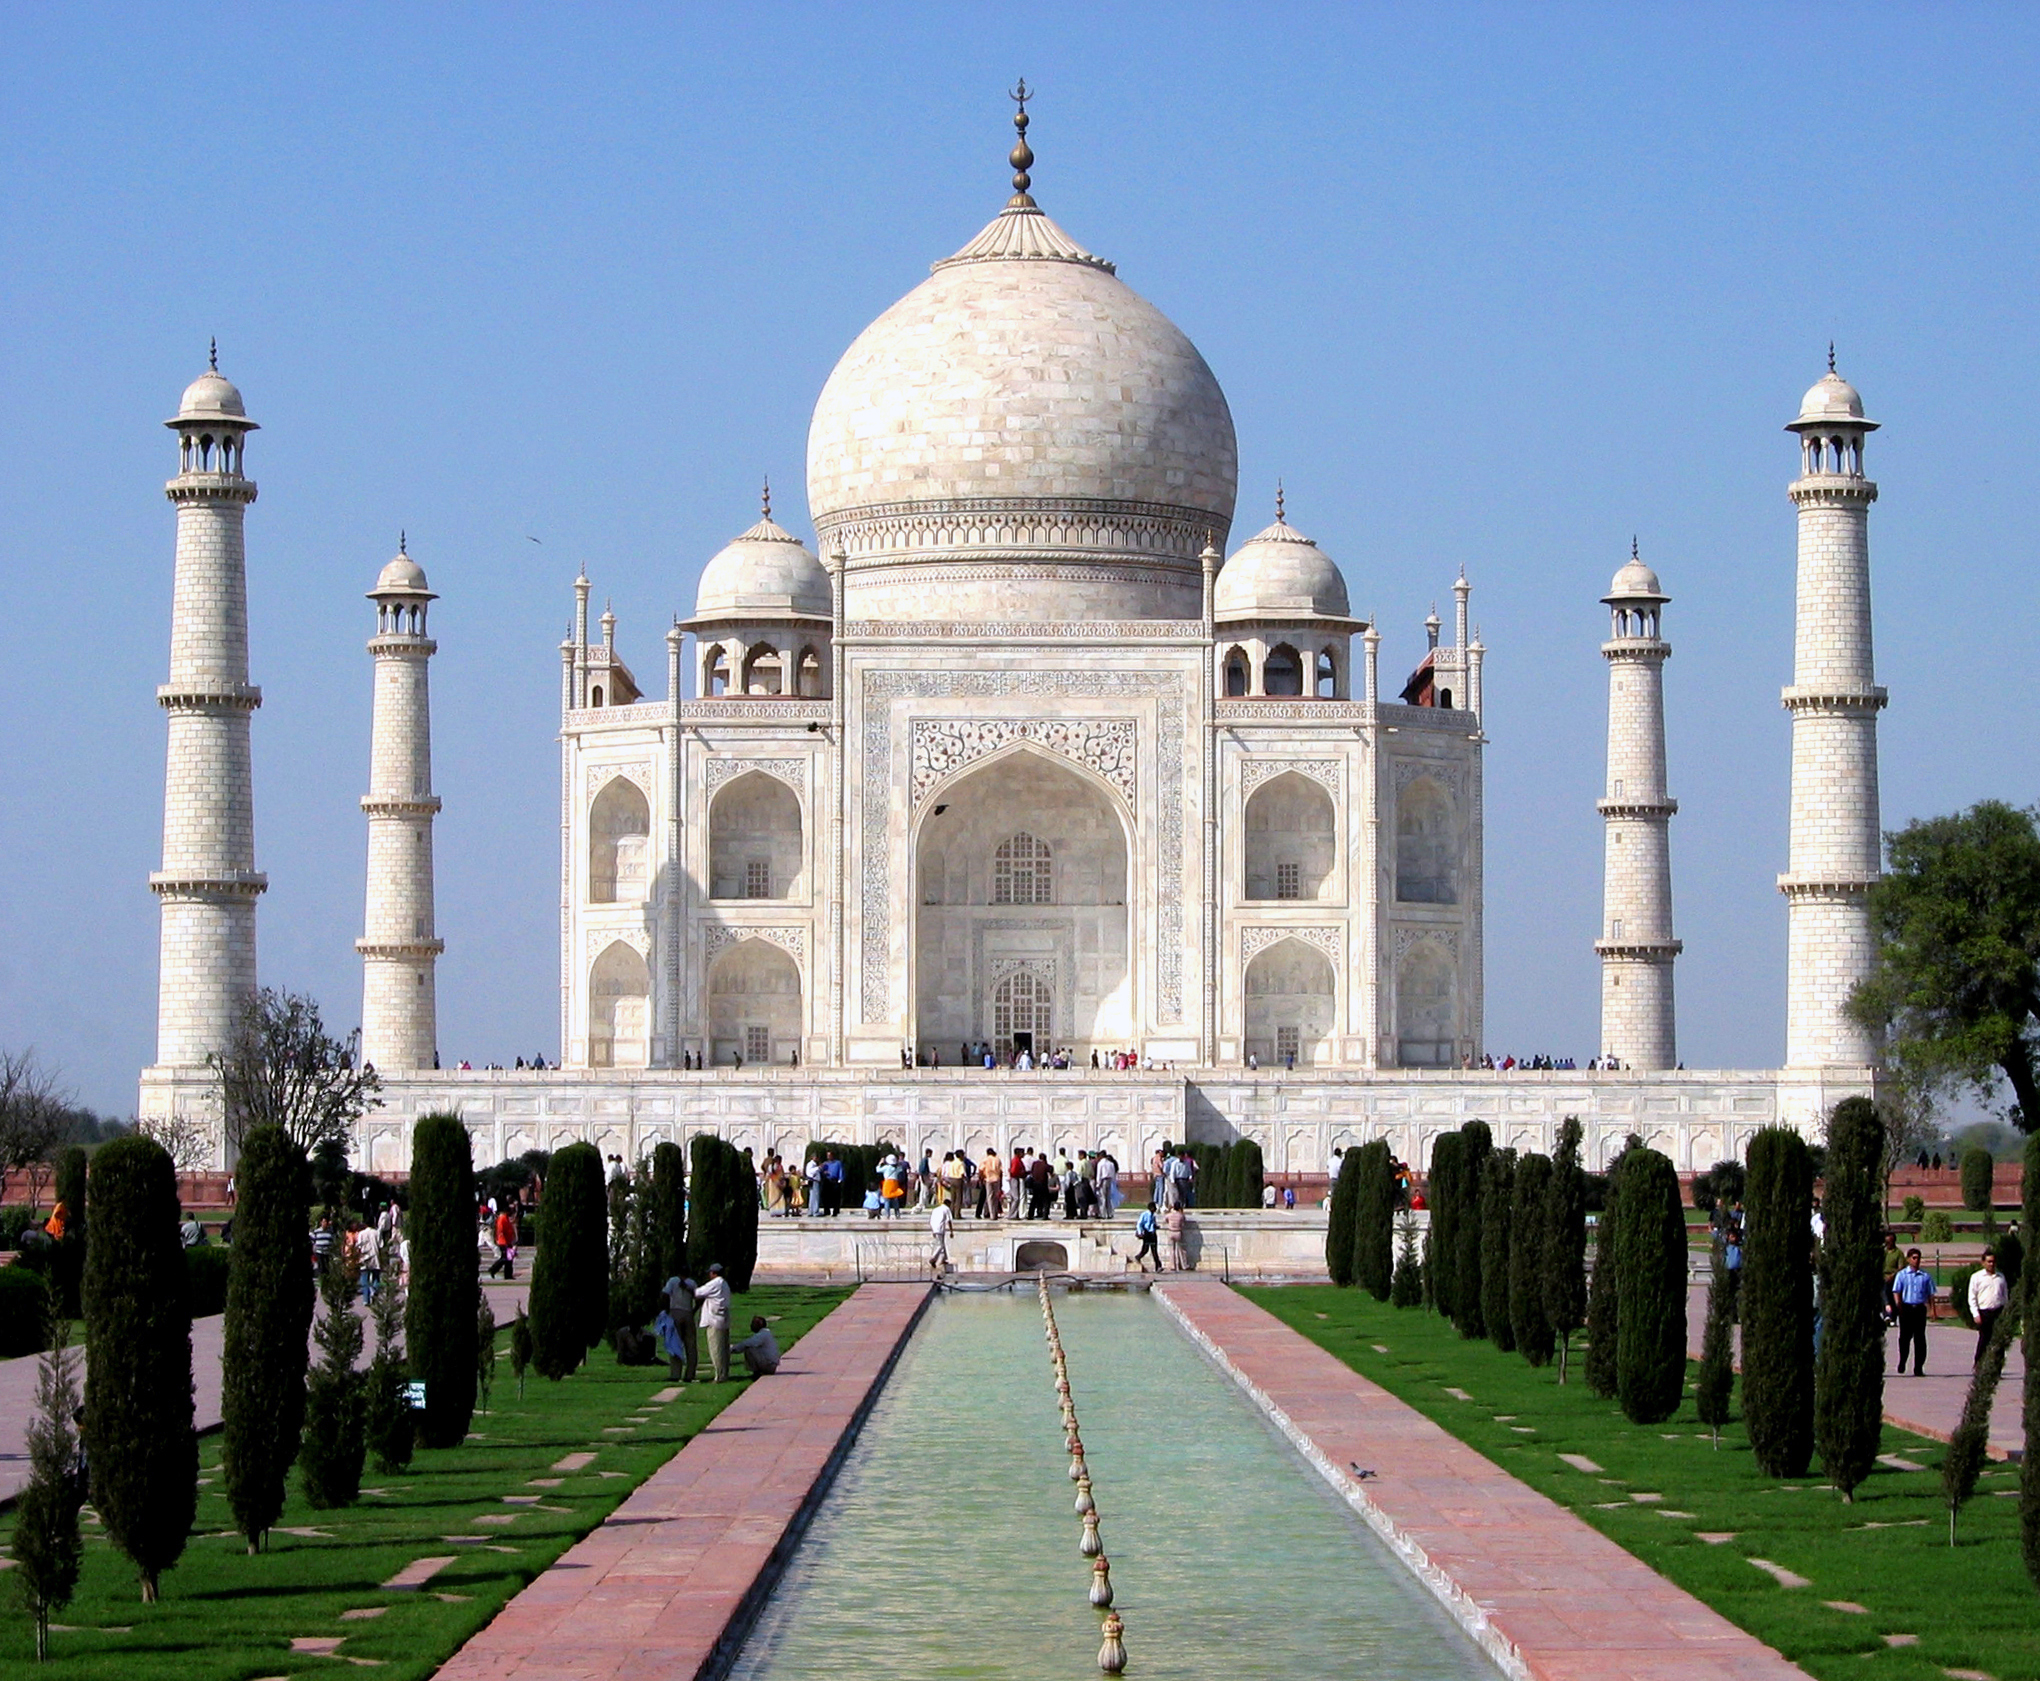
\includegraphics[width=20mm,scale=0.7]{images/taj_mahal.jpg}};}
	\onslide<2->{  \node [right=4.3cm of input_taj.south,anchor=south west] (raw)  { 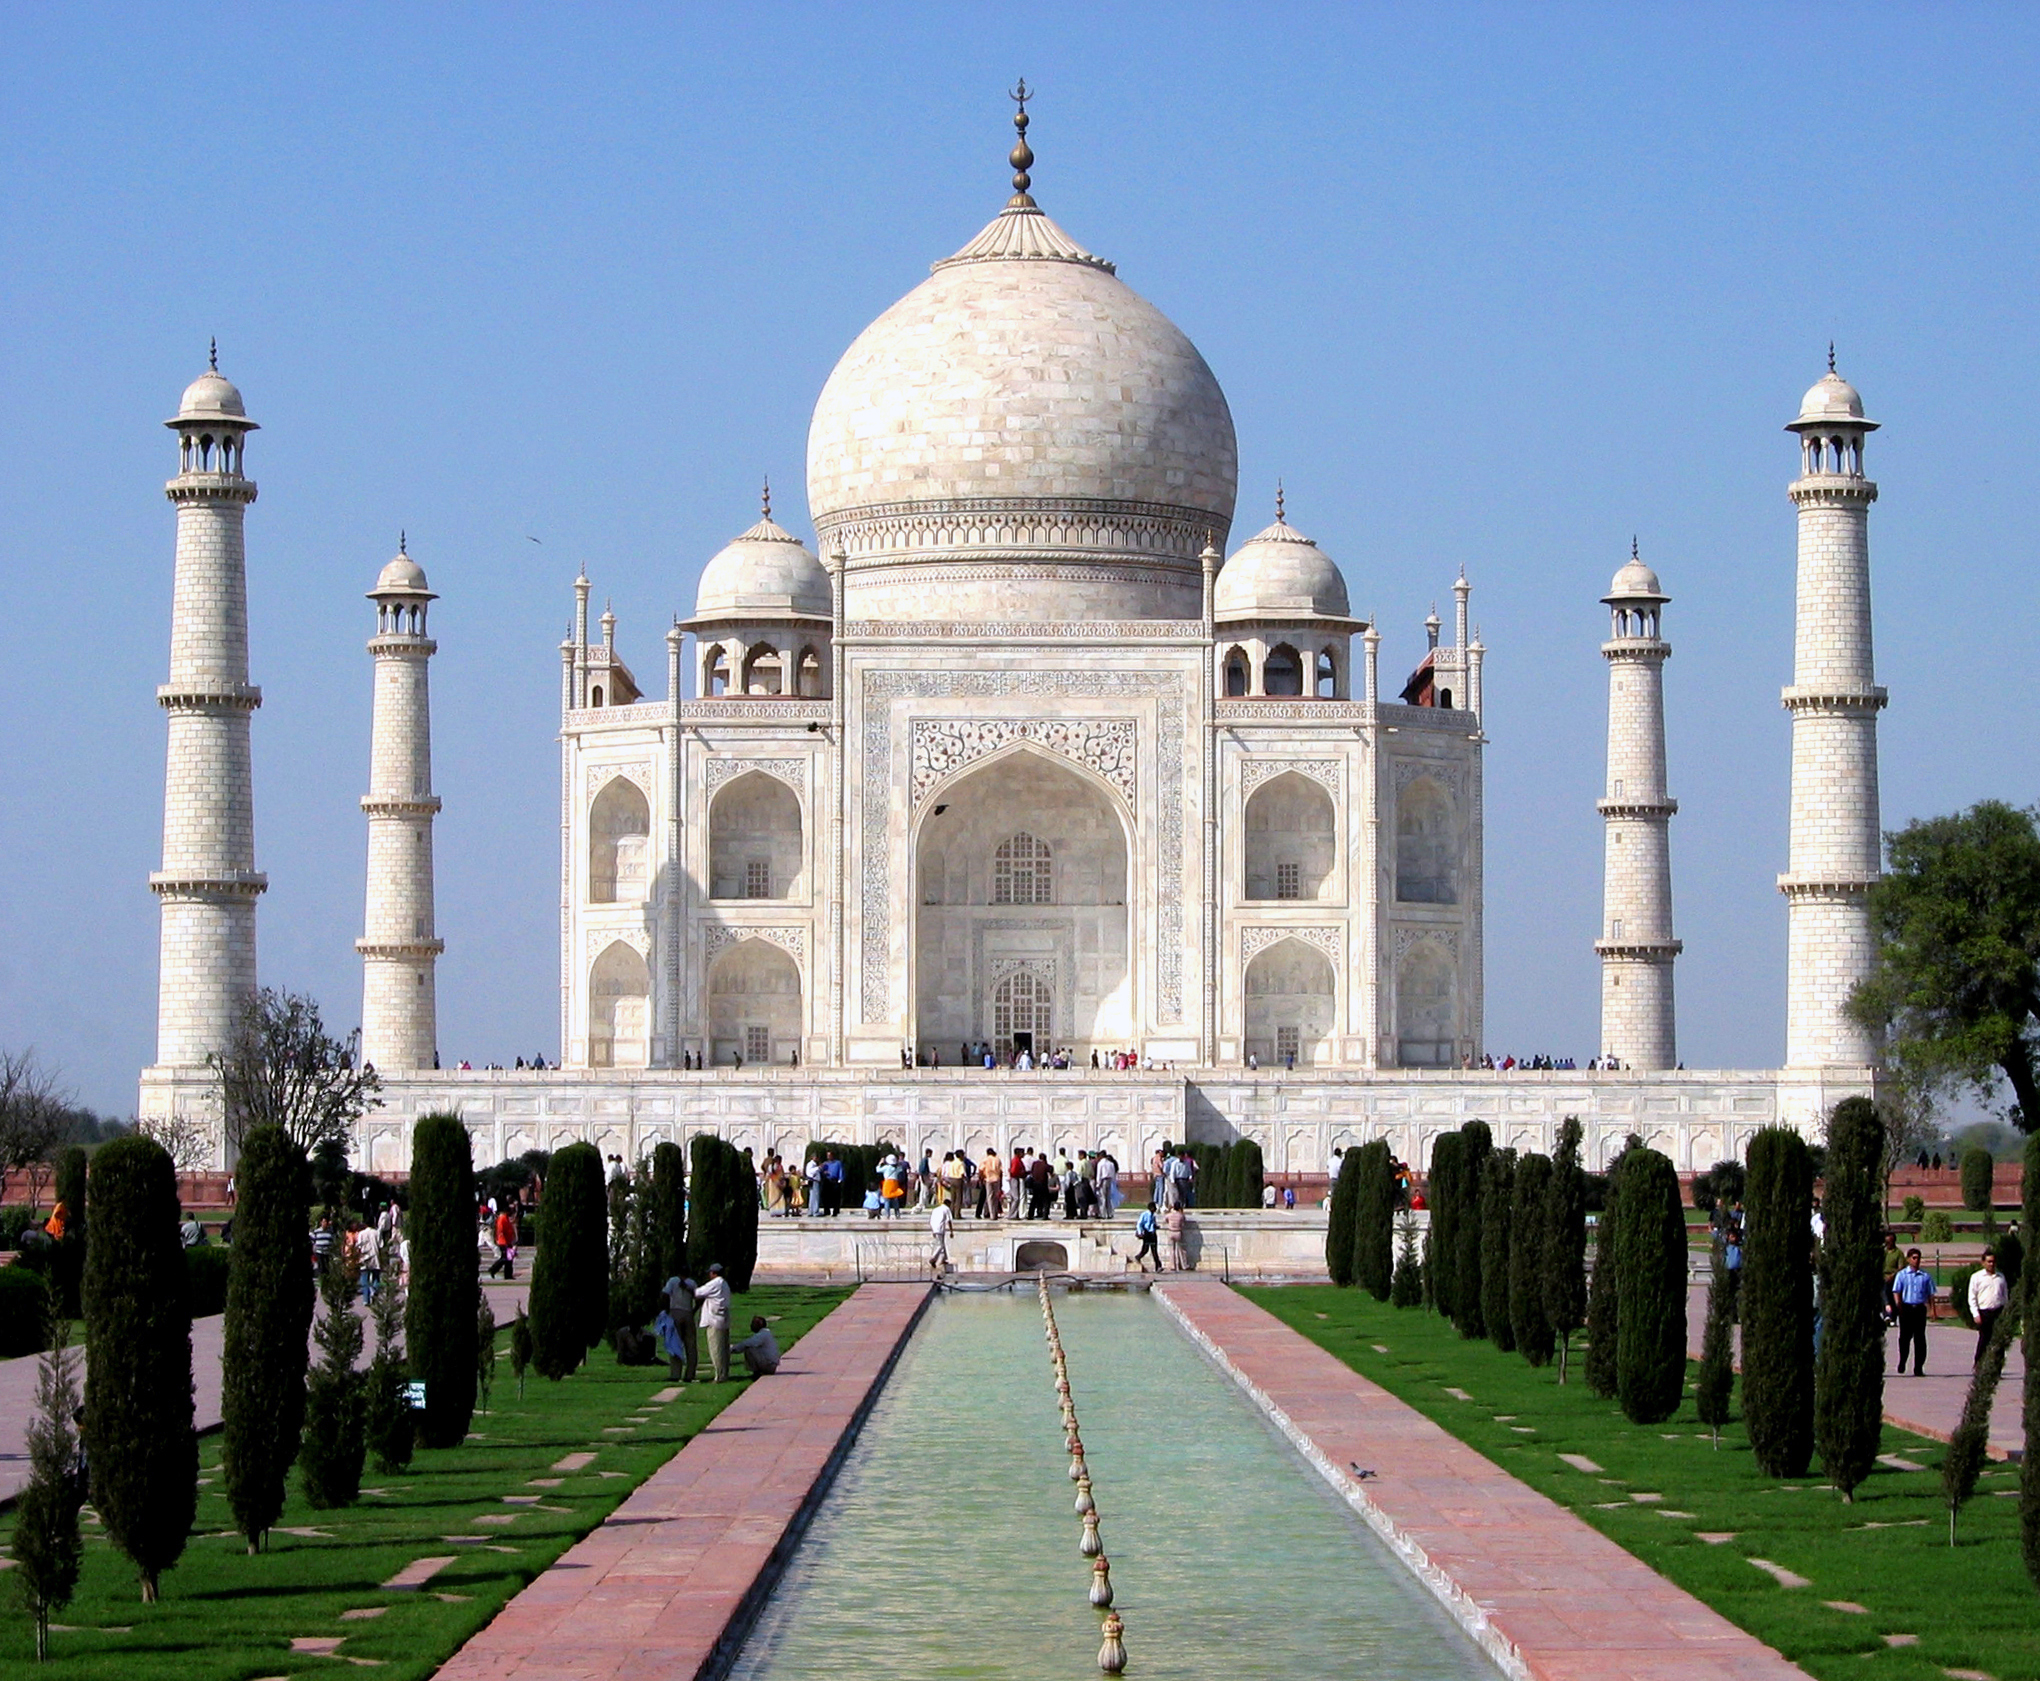
\includegraphics[width=20mm,scale=0.7]{images/taj_mahal.jpg}};

		\node[above of= raw,node distance=1.2cm ] (features)  {Features};
		\draw[->,thick] (input_taj) -- node [midway, above] {\footnotesize{$Raw\,pixels$}} (raw) ;}
	\onslide<3->{\node [right=5cm of raw.center,anchor= center](output_taj){car, bus, \textcolor{blue}{monument}, flower};
		\draw[->,thick] (raw) -- (output_taj) ;}
\end{tikzpicture}